
%(BEGIN_QUESTION)
% Copyright 2014, Tony R. Kuphaldt, released under the Creative Commons Attribution License (v 1.0)
% This means you may do almost anything with this work of mine, so long as you give me proper credit

Calculate the power dissipated by $R_1$ and the voltage between points B and C in this circuit, if we know there is 4.5 volts dropped between points E and F.  There is no need to specify the polarity of the voltage in your answer:

$$\includegraphics[width=15.5cm]{i03046x01.eps}$$

$P_{R1}$ = 

\vskip 10pt

$V_{BC}$ = 

\vskip 10pt

\underbar{file i03046}
%(END_QUESTION)





%(BEGIN_ANSWER)

$P_{R1}$ = 38.36 mW

\vskip 10pt

$V_{BC}$ = 19.77 V

%(END_ANSWER)





%(BEGIN_NOTES)

{\bf This question is intended for exams only and not worksheets!}.

%(END_NOTES)

